%%%%%%%%%%%%%%%%%%%%%%%%%%%%%%%%%%%%%%%%%
% Beamer Presentation
% LaTeX Template
% Version 1.0 (10/11/12)
%
% This template has been downloaded from:
% http://www.LaTeXTemplates.com
%
% License:
% CC BY-NC-SA 3.0 (http://creativecommons.org/licenses/by-nc-sa/3.0/)
%
%%%%%%%%%%%%%%%%%%%%%%%%%%%%%%%%%%%%%%%%%

%----------------------------------------------------------------------------------------
%	PACKAGES AND THEMES
%----------------------------------------------------------------------------------------

\documentclass{beamer}

\mode<presentation> {

% The Beamer class comes with a number of default slide themes
% which change the colors and layouts of slides. Below this is a list
% of all the themes, uncomment each in turn to see what they look like.

\usetheme{default}
%\usetheme{AnnArbor}
%\usetheme{Antibes}
%\usetheme{Bergen}
%\usetheme{Berkeley}
%\usetheme{Berlin}
%\usetheme{Boadilla}
%\usetheme{CambridgeUS}
%\usetheme{Copenhagen}
%\usetheme{Darmstadt}
%\usetheme{Dresden}
%\usetheme{Frankfurt}
%\usetheme{Goettingen}
%\usetheme{Hannover}
%\usetheme{Ilmenau}
%\usetheme{JuanLesPins}
%\usetheme{Luebeck}
%\setheme{Madrid}
%\usetheme{Malmoe}
%\usetheme{Marburg}
%\usetheme{Montpellier}
%\usetheme{PaloAlto}
%\usetheme{Pittsburgh}
%\usetheme{Rochester}
%\usetheme{Singapore}
%\usetheme{Szeged}
%\usetheme{Warsaw}

% As well as themes, the Beamer class has a number of color themes
% for any slide theme. Uncomment each of these in turn to see how it
% changes the colors of your current slide theme.

%\usecolortheme{albatross}
%\usecolortheme{beaver}
%\usecolortheme{beetle}
%\usecolortheme{crane}
%\usecolortheme{dolphin}
%\usecolortheme{dove}
%\usecolortheme{fly}
%\usecolortheme{lily}
%\usecolortheme{orchid}
%\usecolortheme{rose}
%\usecolortheme{seagull}
\usecolortheme{seahorse}
%\usecolortheme{whale}
%\usecolortheme{wolverine}

%\setbeamertemplate{footline} % To remove the footer line in all slides uncomment this line
\setbeamertemplate{footline}[frame number] % To replace the footer line in all slides with a simple slide count uncomment this line

%\setbeamertemplate{navigation symbols}{} % To remove the navigation symbols from the bottom of all slides uncomment this line
}

\usepackage{graphicx} % Allows including images
\usepackage{booktabs} % Allows the use of \toprule, \midrule and \bottomrule in tables
\usepackage{tikz}
\usetikzlibrary{matrix}
\usepackage{listings}
\usepackage{xcolor}
\usepackage{IEEEtrantools}
\usepackage{amsmath}
\usepackage{amssymb}
\usepackage{dsfont}
\usepackage{longtable}

\newcommand{\sep}{-\kern-.6em\raisebox{-.659ex}{*}\ }
\newcommand{\bupd}[1]{=\kern-.6em\{#1\}\ \kern-.9em =\ \kern-.8em\raisebox{-.659ex}{*}\ }
\newcommand{\fupd}{=\kern-.3em=\ \kern-.8em\raisebox{-.659ex}{*}\ }
\newcommand{\nfupd}{=\kern-.6em \backslash\ \kern-.9em=\ \kern-.8em\raisebox{-.659ex}{*}\ }

\newcommand{\bigsep}{\mathop{\scalebox{2.5}{\raisebox{-0.4ex}{$*$}}}}%

\newcommand{\ra}[1] {
  \begin{tikzpicture}
        \node[draw,dashed] {#1};
    \end{tikzpicture}}
    
\newcommand{\inv}[1] {
  \begin{tikzpicture}
        \node[draw] {#1};
    \end{tikzpicture}}
    
\newcommand{\interp}[2]{(#1)(#2)}
\newcommand\sepimp{\mathrel{-\mkern-6mu*}}

\usetikzlibrary{decorations.pathreplacing}

\newcommand\MemoryLayout[1]{
  \begin{tikzpicture}[scale=0.3]
     \draw[thick](0,0)--++(0,1);
     \foreach \pt/\col/\lab [remember=\pt as \tp (initially 0)] in {#1} {
     \if\lab\relax\relax\else
         \draw[thick,decorate, decoration={brace,amplitude=4mm}]
            (-\tp,-0.2)--node[below=4mm]{\lab} (-\pt+2,-0.2);
            \draw[fill=\col] (-\tp,0) rectangle (-\pt+2,1);
       \fi
       \foreach \a in {\tp,...,\pt} {
          \draw(-\a,0) rectangle ++(-1,1);
       }
       \draw[thick](-\pt,0)--++(0,1);
       
     }
     \node at (-4.5,0.6) {\small B};
  \end{tikzpicture}
}

\def\world{\emph{World}}
\def\word{\emph{Word}}

 
\definecolor{codegreen}{rgb}{0,0.6,0}
\definecolor{codegray}{rgb}{0.5,0.5,0.5}
\definecolor{codepurple}{rgb}{0.58,0,0.82}
\definecolor{backcolour}{rgb}{0.95,0.95,0.92}
 
\lstdefinestyle{mystyle}{
    backgroundcolor=\color{backcolour},   
    commentstyle=\color{codegreen},
    keywordstyle=\color{magenta},
    numberstyle=\tiny\color{codegray},
    stringstyle=\color{codepurple},
    basicstyle=\ttfamily\footnotesize,
    breakatwhitespace=false,         
    breaklines=true,                 
    captionpos=b,                    
    keepspaces=true,                 
    numbers=left,                    
    numbersep=5pt,                  
    showspaces=false,                
    showstringspaces=false,
    showtabs=false,                  
    tabsize=2
}
 
\lstset{style=mystyle,xleftmargin=.2\textwidth, xrightmargin=.2\textwidth}

\setbeamercovered{transparent}
\setbeamercolor{alerted text}{fg=red}

\AtBeginSection[]{
  \begin{frame}
  \vfill
  \centering
  \begin{beamercolorbox}[sep=8pt,center,shadow=true,rounded=true]{title}
    \usebeamerfont{title}\insertsectionhead\par%
  \end{beamercolorbox}
  \vfill
  \end{frame}
}

\AtBeginSubsection[]
{
    \begin{frame}
  	\vfill
  	\centering
  	\begin{beamercolorbox}[sep=8pt,center,shadow=true,rounded=true]{title}
    \usebeamerfont{title}\insertsubsectionhead\par%
  	\end{beamercolorbox}
  	\vfill
  \end{frame}
}
%----------------------------------------------------------------------------------------
%	TITLE PAGE
%----------------------------------------------------------------------------------------

\title[Capability Machine in Iris]{Implementing a Capability Machine model into Iris} % The short title appears at the bottom of every slide, the full title is only on the title page

\author{\textbf{A\"{i}na Linn Georges} \hspace{1cm} Alix Trieu \hspace{1cm} Lars Birkedal} % Your name
\institute[Aarhus University] % Your institution as it will appear on the bottom of every slide, may be shorthand to save space
{
Aarhus University \\ % Your institution for the title page
\medskip
\textit{ageorges@cs.au.dk} % Your email address
}
\date{\today} % Date, can be changed to a custom date

\begin{document}

\begin{frame}
\titlepage % Print the title page as the first slide
\end{frame}

\begin{frame}
\frametitle{Introduction}
\centering
\begin{tikzpicture}
    \node<1-3> (img1) {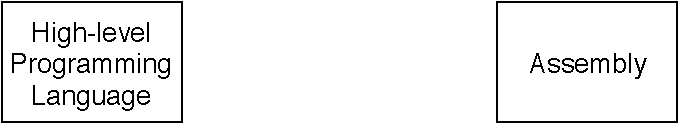
\includegraphics[scale=0.7]{images/sec_1.pdf}};
    \node<4> (img2) {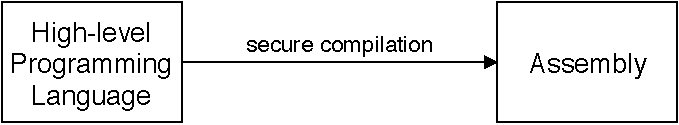
\includegraphics[scale=0.7]{images/sec_2.pdf}};
\end{tikzpicture}
\\[1cm]
\begin{itemize}
	\item<2-> Local state encapsulation
	\item<3-> Well bracketed control flow
\end{itemize}
\end{frame}

\begin{frame}
\frametitle{Layers of Abstraction}

\begin{block}{Programming Languages}
	\begin{itemize}
		\item<2-> Local State Encapsulation
		\item<3-> Well Bracketed Control Flow
	\end{itemize}
\end{block}

\begin{block}{Assembly Language}
	\begin{itemize}
		\item<4-> Programs lie in Memory, Program Counter, ...
		\item<5-> Arbitrary Pointer Manipulation
		\item<6-> Arbitrary Jumps
	\end{itemize}
\end{block}

\begin{block}{Machine Code}
	\begin{itemize}
		\item<7-> Instruction Decoding, Cache, etc. 
	\end{itemize}
\end{block}

\begin{block}{$\cdots$}
\end{block}

\end{frame}

%----------------------------------------------------------------------------------------
%	PRESENTATION SLIDES
%----------------------------------------------------------------------------------------

\begin{frame}
\frametitle{Overview} % Table of contents slide, comment this block out to remove it
\tableofcontents[hideallsubsections]
 % Throughout your presentation, if you choose to use \section{} and \subsection{} commands, these will automatically be printed on this slide as an overview of your presentation
\end{frame}

%------------------------------------------------
\section{Capability Machines} % Sections can be created in order to organize your presentation into discrete blocks, all sections and subsections are automatically printed in the table of contents as an overview of the talk
%------------------------------------------------


\begin{frame}
\frametitle{Capability Machine}

\uncover<5->{\textbf{Capability: } An unforgeable token of authority
\\[1cm]}
\begin{columns}[c]

\column{.45\textwidth} % Left column and width
\begin{tikzpicture}
    \node<1> (img1) {
\includegraphics[scale=0.7]{images/cap_1.pdf}};
    \node<2> (img2) {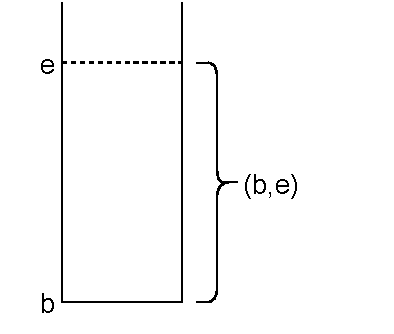
\includegraphics[scale=0.7]{images/cap_2.pdf}};
    \node<3> (img3) {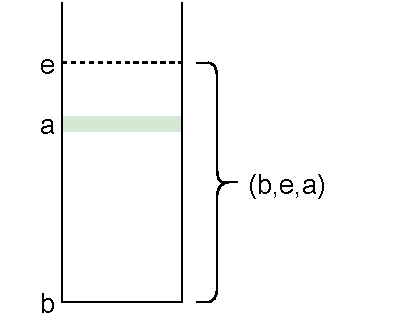
\includegraphics[scale=0.7]{images/cap_3.pdf}};
    \node<4-> (img4) {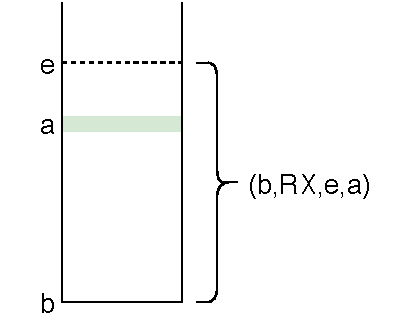
\includegraphics[scale=0.7]{images/cap_4.pdf}};
\end{tikzpicture}

\column{.5\textwidth} % Right column and width
\uncover<4->{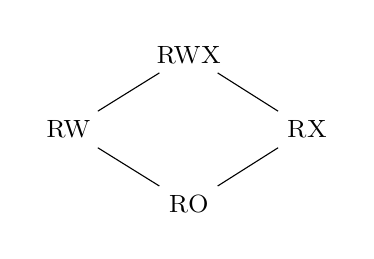
\begin{tikzpicture}

\matrix (a) [matrix of math nodes, ampersand replacement=\&, column sep=0.6cm, row sep=0.5cm]{
\& \textsc{\small RWX} \&\\
\textsc{\small RW}  \& \& \textsc{\small RX}  \\
\& \textsc{\small RO} \&\\};

\foreach \i/\j in {1-2/2-1, 1-2/2-3, 2-1/3-2, 2-3/3-2}
    \draw (a-\i) -- (a-\j);
%
\end{tikzpicture}}

\end{columns}
\end{frame}

%------------------------------------------------
\subsection{Enforcing Local Stack Encapsulation using Capabilities} % A subsection can be created just before a set of slides with a common theme to further break down your presentation into chunks

\begin{frame}[fragile]
\frametitle{Capability Safety}
\textbf{Local State Encapsulation}
\\[1cm]
\begin{columns}[c]

\column{.45\textwidth} % Left column and width
\begin{tikzpicture}
    \node<1> (img1) {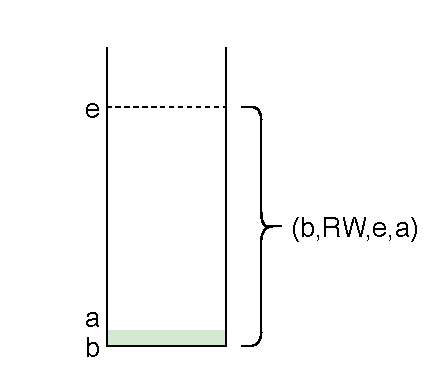
\includegraphics[scale=0.7]{images/wbcf_1.pdf}};
    \node<2> (img2) {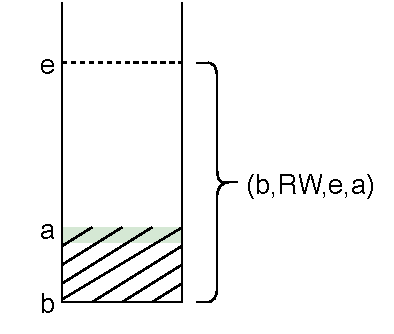
\includegraphics[scale=0.7]{images/wbcf_2.pdf}};
    \node<3> (img3) {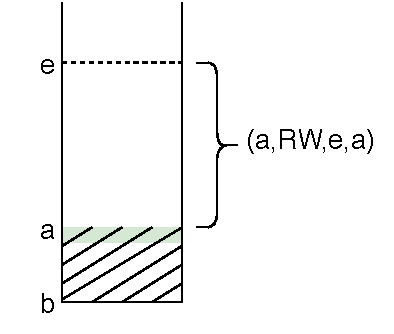
\includegraphics[scale=0.7]{images/wbcf_3.pdf}};
\end{tikzpicture}

\column{.5\textwidth} % Right column and width
\begin{center}
\begin{lstlisting}
push r_stk 1
scall r 
pop r_stk r_1
assert r_1 1
halt
\end{lstlisting}
\end{center}


\end{columns}
\end{frame}

%------------------------------------------------
\subsection{Enforcing Well Bracketed Control Flow using Capabilities} % A subsection can be created just before a set of slides with a common theme to further break down your presentation into chunks

\begin{frame}[fragile]
\frametitle{Capability Safety}
\textbf{Well Bracketed Control Flow}
\\[1cm]
\begin{columns}[c]

\column{.45\textwidth} % Left column and width
\begin{tikzpicture}
    \node<1> (img1) {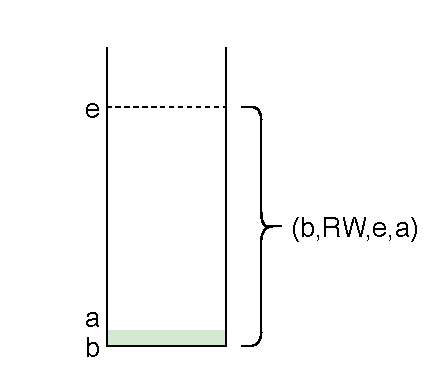
\includegraphics[scale=0.7]{images/wbcf_1.pdf}};
    \node<2> (img2) {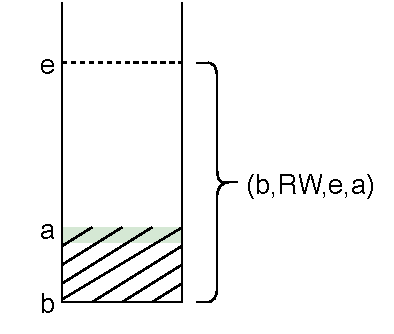
\includegraphics[scale=0.7]{images/wbcf_2.pdf}};
    \node<3> (img3) {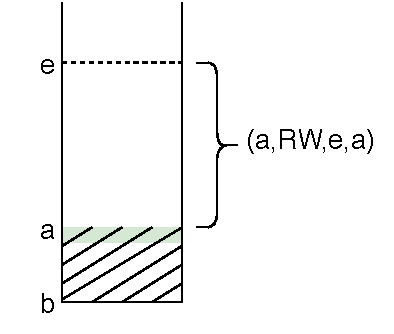
\includegraphics[scale=0.7]{images/wbcf_3.pdf}};
    \node<4> (img4) {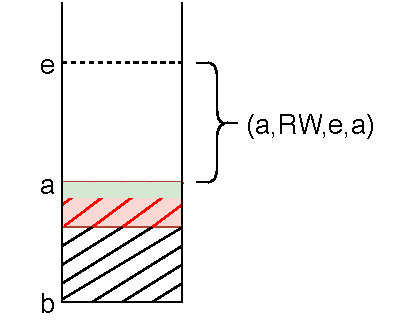
\includegraphics[scale=0.7]{images/wbcf_4.pdf}};
    \node<5> (img5) {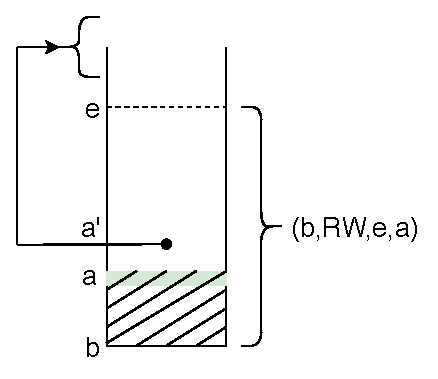
\includegraphics[scale=0.7]{images/wbcf_5.pdf}};
    \node<6> (img6) {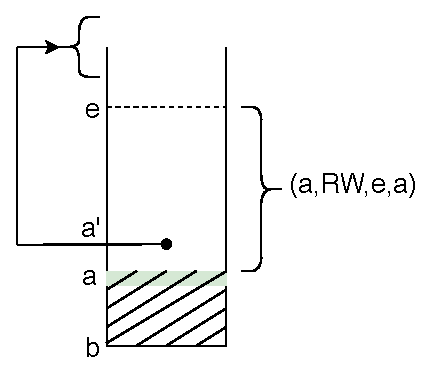
\includegraphics[scale=0.7]{images/wbcf_6.pdf}};
\end{tikzpicture}

\column{.5\textwidth} % Right column and width
\begin{center}
\begin{lstlisting}
push r_stk 1
scall r
pop r_stk r_1
assert r_1 1
push r_stk 2
scall r 
halt
\end{lstlisting}
\end{center}

\end{columns}
\end{frame}

%------------------------------------------------
\subsection{Local Capabilities}
\begin{frame}
\frametitle{Local Capabilities}

\begin{center} (p,\textbf{Local},b,e,a) \hspace{2cm} (p,\textbf{Global},b,e,a) \end{center}

\uncover<2->{

\begin{tikzpicture}

\matrix (a) [matrix of math nodes, ampersand replacement=\&, column sep=0.6cm, row sep=0.5cm]{
\& \& \textsc{\small RWLX} \& \& \& \\
\& \textsc{\small RWX} \& \& \textsc{\small RWL} \& \& \\
\textsc{\small RX} \& \& \textsc{\small RW}  \&  \\
\& \textsc{\small RO} \& \\};

\foreach \i/\j in {1-3/2-2, 1-3/2-4, 2-2/3-1, 2-4/3-3, 2-2/3-3, 3-1/4-2, 3-3/4-2}
    \draw (a-\i) -- (a-\j);
%
\end{tikzpicture}
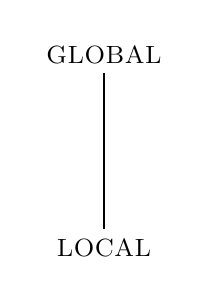
\begin{tikzpicture}

\matrix (a) [matrix of math nodes, ampersand replacement=\&, column sep=0.6cm, row sep=0.5cm]{
\textsc{\small GLOBAL}\\ \\ \\ \\
\textsc{\small LOCAL}\\};

\foreach \i/\j in {1-1/5-1}
    \draw (a-\i) -- (a-\j);
%
\end{tikzpicture}
}
\uncover<3>{
\begin{center} well-bracketed \hspace{2cm} not well-bracketed \end{center}}

\end{frame}

\begin{frame}
\frametitle{Calling Convention}
\begin{tikzpicture}
    \node<1> (img1) {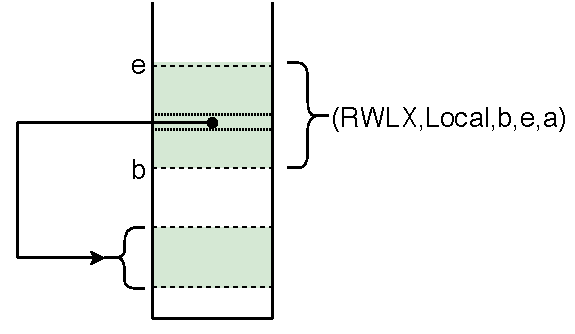
\includegraphics[scale=0.7]{images/calling_1.pdf}};
    \node<2> (img2) {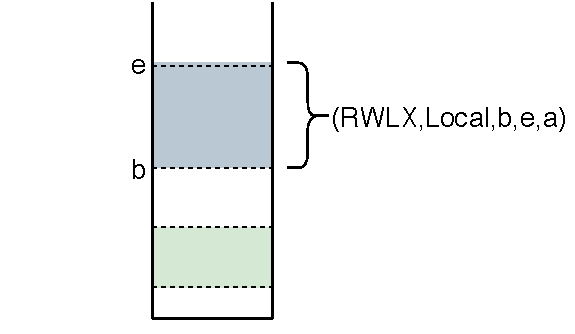
\includegraphics[scale=0.7]{images/calling_2.pdf}};
\end{tikzpicture}

\begin{longtable}[c]{|l|l|}
\hline
\texttt{r\_stk} & $(RWLX,Local,b,e,a)$ \\ \hline
\endfirsthead
%
\endhead
\end{longtable}

\end{frame}

%------------------------------------------------
\section{Reasoning about Capability Safety}

\begin{frame}
\frametitle{Expressing Capability Safety}

\begin{itemize}
	\item<2-> using a Program Logic 
	\item<3-> using a logical relation to capture invariants on the type system
	\item<4-> \textbf{using a logical relation on an \emph{untyped} (or \emph{uni-typed}) language to capture semantic properties of the language}
\end{itemize}

\end{frame}

\begin{frame}
\frametitle{Expressing Capability Safety}

\begin{itemize}
	\item<1-> \textbf{using a logical relation on an \emph{untyped} (or \emph{uni-typed}) language to capture semantic properties of the language}
	\begin{enumerate}
		\item<2-> embed the language into Iris
		\item<3-> define a program logic by proving Hoare Triples
		\item<4-> define the logical relation
		\item<5-> prove the fundamental theorem of logical relations
		\item<6-> use the logical relation to prove examples that rely on local state encapsulation and well-bracketed control flow with calls to unknown adversary
	\end{enumerate}
\end{itemize}

\end{frame}

%------------------------------------------------
\section{Program Logic}
%------------------------------------------------

\begin{frame}
\frametitle{Abstract Instructions}

$$(reg,mem) \rightarrow (reg',mem')$$
%
\begin{itemize}
	\item<2-> \textsf{Instr Executable}
	\item<3-> \textsf{Instr Halted} \uncover<5->{$\rightarrow$ \textsf{HaltedV}}
	\item<4-> \textsf{Instr Failed} \uncover<5->{$\rightarrow$ \textsf{FailedV}}
\end{itemize}

\end{frame}

%------------------------------------------------
\subsection{A Capability Points-to Predicate}
\begin{frame}
\frametitle{Points-to Predicate with Permissions}

\begin{align*}
	a \mapsto_a[RWL] w \only<2->{&\fupd a \mapsto_a[RWL] ((p,Local),b,e,l) \\}
	\only<3->{&\fupd a \mapsto_a[RW] ((p,Local),b,e,l) \\}
	\only<4->{&\nfupd a \mapsto_a[RW] ((p',Local),b',e',l') \\}
\end{align*}

\end{frame}

%------------------------------------------------
\section{Proving Hoare Triples}

%------------------------------------------------
\subsection{Successful Execution}

\begin{frame}
\frametitle{Hoare Triples of the Program Logic: Success}

\begin{align*}
&decode(w) = \textsf{Load dst src} \\
\wedge &\textsf{ isCorrectPC }((p_{pc},g_{pc}),b_{pc},e_{pc},a_{pc}) \\
\wedge &\textsf{ readAllowed } p_{src} ~\wedge~  \textsf{withinBounds } (b_{src},e_{src},a_{src})\\ \\
\{\{\{&~ \alert<2>{\textsf{PC} \mapsto_r ((p_{pc},g_{pc}),b_{pc},e_{pc},a_{pc})} * a_{pc} \mapsto_a[p_{pc}] w \\
&* \alert<3>{dst \mapsto_r w_{dst}} * src \mapsto_r ((p_{src},g_{src}),b_{src},e_{src},a_{src}) \\
&* a_{src} \mapsto_a[p_{src}] w_{src} \}\}\} \\
&\textsf{Instr Executable} \\
\{\{\{&~  \alert<2>{\textsf{PC} \mapsto_r ((p_{pc},g_{pc}),b_{pc},e_{pc},a_{pc} + 1)}
			  * a_{pc} \mapsto_a[p_{pc}] w
			  \\&* \alert<3>{dst \mapsto_r w_{src}}
			  * src \mapsto_r ((p_{src},g_{src}),b_{src},e_{src},a_{src})
			   \\&* a_{src} \mapsto_a[p_{src}] w_{src} \}\}\}
\end{align*}

\end{frame}

%------------------------------------------------
\subsection{Failed Execution}

\begin{frame}
\frametitle{Hoare Triples of the Program Logic: Failure}

\begin{align*}
&decode(w) = \textsf{Load dst src} \\
\wedge &\textsf{ isCorrectPC }((p_{pc},g_{pc}),b_{pc},e_{pc},a_{pc}) \\
\wedge &~\alert<2>{\neg \textsf{readAllowed } p_{src}} ~\vee~ \neg \textsf{withinBounds } (b_{src},e_{src},a_{src})\\
\{\{\{&~\textsf{PC} \mapsto_r ((p_{pc},g_{pc}),b_{pc},e_{pc},a_{pc}) * a_{pc} \mapsto_a[p_{pc}] w \\
&* src \mapsto_r ((p_{src},g_{src}),b_{src},e_{src},a_{src}) \}\}\} \\
&\textsf{Instr Executable} \\
\{\{\{&~ \alert<2>{\textsf{FailedV}}, \top \}\}\}
\end{align*}

\end{frame}

%------------------------------------------------
\section{A Unary Logical Relation for Reasoning about Semantic Properties of an Untyped Language}
%------------------------------------------------

%------------------------------------------------
\subsection{The Value Relation}

\begin{frame}[fragile]
\frametitle{The Value Relation}
\begin{center}
\textbf{A unary logical relation of an un-typed language}
\end{center}

$$\mathcal{V} : \only<2->{{\color{red}World} \rightarrow~} 
			Word \rightarrow iProp~\Sigma $$
\begin{itemize}
	\item<2-> {\color{red} World}: A collection of state transition systems\\
	to reason about \textit{local state}\\
					
\end{itemize}

\uncover<3->{
\begin{align*}
  		\mathcal{V}\interp{W}{z} \triangleq&~\exists z' \in \mathds{Z}. z = z' \\
  		\mathcal{V}\interp{W}{((\text{\tiny{RO}},g),b,e,a)} \triangleq&~\textsf{read\_write\_cond}(\textsf{RO,b,e}) \\
  		\mathcal{V}\interp{W}{((\text{\tiny{RX}},g),b,e,a)} \triangleq&~\textsf{read\_write\_cond}(\textsf{RX,b,e}) \\&* ~\square~\textsf{exec\_cond(W)(\textsf{RX,g,b,e})}
 	\end{align*}}

\end{frame}

%------------------------------------------------
\subsection{The Execute Condition}

\begin{frame}
\frametitle{The Execute Condition}

\begin{equation*}
\textsf{exec\_cond(W)(\textsf{p,g,b,e})} \triangleq \begin{cases}
\forall a \in [b~e], W' \sqsubseteq_{pub} W.\\
~\rhd~\mathcal{E}\interp{W'}{((p,g),b,e,a)} &g = Local\\ \\
\forall a \in [b~e], W' \sqsubseteq_{priv} W.\\
~\rhd~\mathcal{E}\interp{W'}{((p,g),b,e,a)} &g = Global\\
\end{cases}
\end{equation*}

\end{frame}

%------------------------------------------------
\subsection{The Expression Relation}

\begin{frame}
\frametitle{The Expression Relation}

 	\begin{align*}
 		\mathcal{E}\interp{W}{pc} \triangleq&~\forall r, \mathcal{R}(W)(r) ~*~{\only<2->{\color{red}} \textsf{context}(W)(r[\textsf{\small PC}:=pc])}\\
 		&\sep~\textsc{WP}~\textsf{Seq (Instr Executable)}~\\
 		&\hspace{1cm}\{ v, v = HaltedV \implies \exists W' r', W' \sqsubseteq_{priv} W \\
 		&\hspace{1cm}* {\only<2->{\color{red}}\textsf{context}(W')(r')}\}
 	\end{align*}

\only<2->{
\begin{align*}
	{\color{red} \textsf{context}(W)(r) =~\only<2>{?}} &\only<3->{(\bigsep_{r_i \mapsto w \in r} r_i \mapsto_r w) \wedge \textsf{full\_map } r}\\
	\only<4->{&* \textsf{na\_inv } \gamma_{na} \top \\ }
	\only<5->{&* \textsf{sts\_full } W \\ }
	\only<6->{&* \textsf{region } W \\ }
\end{align*}
}

\end{frame}

%------------------------------------------------
\section{The Fundamental Theorem of Logical Relations}

\begin{frame}
\frametitle{The Fundamental Theorem of logical relations}
\begin{center}
If we can read a region, and every word in that region is safe, then we can safely execute it
\end{center}
\end{frame}
	
\begin{frame}
\begin{itemize}
	\item<2-> "If we can read a region" : $p = \textsc{\small RX} \vee p = \textsc{\small RWX} \vee p = \textsc{\small RWLX}$
	\item<3-> "and every word in that region is safe": $\textsf{read\_write\_cond }(p,b,e)$
	\item<4-> "then we can safely execute it": $\mathcal{E}\interp{W}{((p,g),b,e,a)}$
\end{itemize}

\begin{align*}
	&(p = \textsc{\small RX} \vee p = \textsc{\small RWX} \vee p = \textsc{\small RWLX}) \implies\\
	&\textsf{read\_write\_cond }(p,b,e) \implies \mathcal{E}\interp{W}{((p,g),b,e,a)}
\end{align*}
\end{frame}

%------------------------------------------------
\section{Reasoning about Unknown Code}

\begin{frame}[fragile]
\frametitle{Reasoning about Unknown Code}
\textbf{We use the fundamental theorem to reason about calls to an unknown adversary}

\begin{columns}[c]

\column{.45\textwidth} % Left column and width
\begin{tikzpicture}
    \node (img3) {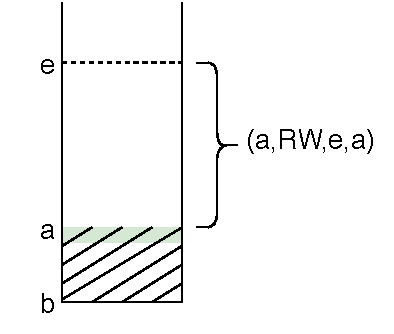
\includegraphics[scale=0.7]{images/wbcf_3.pdf}};
\end{tikzpicture}

\column{.5\textwidth} % Right column and width
\begin{center}
\begin{lstlisting}
push r_stk 1
scall r 
pop r_stk r_1
assert r_1 1
halt
\end{lstlisting}
\end{center}

\end{columns}

\begin{align*}
 		\mathcal{E}\interp{W}{pc} \triangleq&~\forall r, \mathcal{R}(W)(r) ~*~{\textsf{context}(W)(r[\textsf{\small PC}:=pc])}\\
 		&\sep~\textsc{WP}~\textsf{Seq (Instr Executable)}~\\
 		&\hspace{1cm}\{ v, v = HaltedV \implies \exists W' r', W' \sqsubseteq_{priv} W \\
 		&\hspace{1cm}* {\textsf{context}(W')(r')}\}
 	\end{align*}

\end{frame}

%------------------------------------------------
%\section{Conclusion}
%------------------------------------------------

\begin{frame}
\frametitle{Conclusion}

\begin{itemize}
	\item Embed a capability machine into Iris
	\item Define its program logic 
	\item Mechanize a unary logical relation for an untyped capability machine language
	\item Prove the fundamental theorem of logical relations
	\item Reason about examples that rely on Local Stack Encapsulation and Well-Bracketed Control Flow with calls to an unknown adversary
\end{itemize}

\end{frame}


%------------------------------------------------

\begin{frame}
\frametitle{References}
\footnotesize{
\begin{thebibliography}{99} % Beamer does not support BibTeX so references must be inserted manually as below
\bibitem[Skorstensgaard, 2018]{p1} Lau Skorstengaard, 
Dominique Devriese, 
and Lars Birkedal (2018)
\newblock Reasoning About a Machine with Local Capabilities
\newblock ESOP \emph{Programming Languages and Systems} 475--501.

\bibitem[Dreyer, 2012]{p2} Derek Dreyer, Georg Neis, Lars Birkedal (2012)
\newblock The impact of higher-order state and control effects on local relational reasoning
\newblock \emph{Journal of Functional Programming} 22(4-5) 477--528.

\bibitem[Dreyer, 2011]{p3} Derek Dreyer, Amal Ahmed, Lars Birkedal (2011)
\newblock Logical Step-Indexed Logical Relations
\newblock \emph{LMCS} 7(2:16).

\end{thebibliography}
}
\end{frame}

%----------------------------------------------------------------------------------------

\end{document} 